Aggregate programming \cite{Aggregate01} is an emerging framework and paradigm for the development of Collective Adaptive Systems. It is based on a layered architecture with which the developers can describe the system as an "aggregate" of heterogeneous devices, abstracting from the details of coordination and comunication and instead focusing on the collective behavior. The foundation of the Aggregate Programming is the \textit{field calculus} \cite{FieldCalculus}, a functional programming model that unifies local and aggregate semantic.

\section{Field Calculus}

The \textit{field calculus} is a programming model based on the notion of \textit{computational fields} \cite{Field} (or simply \textit{field}). A \textit{field} is a distributed map from devices to computation objects across time. Therefore the field calculus describes how to build those distributed structure and reusable blocks of computation from fields to fields.

The computational model of the field calculus is based on a network of devices that executes a common program in asyncronous rounds. These devices comunicate with neighbour devices following a dynamic (physical or logical) proximity relation. From the local point of view of a single device every round of execution is composed by the following steps: (i) all the information from sensors and the device memory are collected, (ii) from the most recent messages from neighbouring devices a \textit{neighbouring field} is formed, (iii) the program is executed with the collected information, (iv) the results of the computation are stored in the device memory and shared to the neighbouring devices as a message. A device $\deviceId$ is said to "fire" when it runs a round of execution.

From the aggregate point of view the whole computation can be seen as  a space-time data structure, called \textit{field evolution} $\feS$.  Every execution is represented by a point in space-time called an \textit{event} $\eventId$, $\feS$ is then a map from events to computations values. As described in \cite{Universality} the causal relationship between events can be formalized by an \textit{event structure}.

An \textit{event structure} $\EventS$ is a countable set of events \textit{E} togheter with a neighbouring relation $\neigh \subseteq E \times E $ and a causality relation $< \subseteq E \times E$, such that the transitive closure of $\neigh$ forms the irreflexive partial order $<$ and the set $\bp{\eventId' \in E | \eventId' < \eventId }$ is finite for all $\eventId$ (i.e., $<$ is locally finite). Every $\neigh$ relation represent a message sent from the head neighbour to the tail neighbour with the results of the head computation.

\begin{figure}
\centering
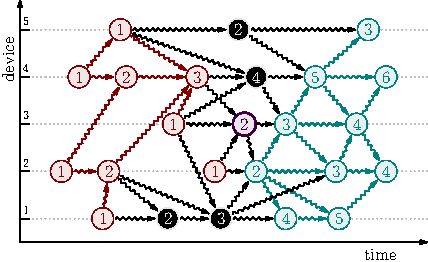
\includegraphics[width=0.8\textwidth]{imgs/structure.pdf}	
\caption{Example of a space-time event structure from \cite{Share}, comprising events (circles), neighbour relations (arrows) and devices (ordinate axis). With respect to the doubly-circled event, the red events are its causal past, the cyan its causal future and the black ones are concurrent.}
\label{fig:eventstructure}
\end{figure}

Figure \ref{fig:eventstructure} shows an example of an event structure, showing the relations among events.

The field calculus is a tiny functional language based on a set of abstract operators for the field computations. In this thesis only an higher-order extension of the field calculus, called \textit{higher-order field calculus (HFC)} \cite{FieldCalculus}, will be considered. HFC extends the field calculus by treating function as first-class values and will be simply refered to as \textit{field calculus} from now on.

\begin{figure}[t]
\centering
\centerline{\framebox[\linewidth]{$
        \begin{array}{lcl@{\hspace{18mm}}r}
                \PROGRAM & \BNFcce & \overline{\FUNCTION}  \; \e
                &{ \mbox{\footnotesize program}}
                \\[3pt]
                \FUNCTION & \BNFcce &  \defK \,\; \fname (\overline{\xname}) \; \{ \e \}
                &{ \mbox{\footnotesize function declaration}}
                \\[3pt]
                \e & \BNFcce &  \xname \;\BNFmid\; \anyvalue \;\BNFmid\; \e(\overline\e) \;\BNFmid\; \fifK (\e) \{\e\} \elseK \{\e\} \;\BNFmid &{ \mbox{\footnotesize expression}} \\
                && \nbrK\{\e\} \;\BNFmid\; \repK(\e)\{ (\xname) \ftoSym \e \} \; \BNFmid \; \\
                && \shareK(\e)\{(\xname) \ftoSym \e \}
                \\[3pt]
                \anyvalue & \BNFcce &  \lvalue \; \BNFmid \; \fvalue
                &{ \mbox{\footnotesize value}}
                \\[3pt]
              \lvalue & \BNFcce &  \dcOf{\dc}{\overline\lvalue} \; \BNFmid \; \funvalue
                &{ \mbox{\footnotesize local value}}
                \\[3pt]
                \fvalue & \BNFcce &  \envmap{\overline\deviceId}{\overline\lvalue}
                &{ \mbox{\footnotesize neighbouring field value}}
                \\[3pt]
                \funvalue & \BNFcce &  \fname \; \BNFmid \; \bname \;\BNFmid\; (\overline{\xname}) \toSym{\name} \e 
                &{ \mbox{\footnotesize function value}}
                \\[3pt]
        \end{array}
        $}
}
\caption{Abstract syntax of the field calculus from \cite{FieldCalculus, Share}} \label{fig:fcsyntax}
\end{figure}

The set of abstract operators is provided in figure \ref{fig:fcsyntax}. Following the notation of \cite{FeatherJava} the overbar denotes a sequence, for example $\overline{\e}$  denotes a (possible empty) sequence of expressions $\e_1, \e_2, \dots, \e_n$.

A program is then a sequence of function definition followed by a main expression $e$, which defines the behavior of the aggregate. 

A function declaration defines a function named $d$ with a sequence of variable names $\overline{\xname}$ and a body of the function consisting in an expression $e$. The defined functions can be recursive.

An expression can be:
\begin{itemize}
\item a variable $\xname$ referring a function parameter
\item a function call $\e(\overline{\e})$, where $\e$ evaluates to a field of functions $\funvalue$, $\overline{\e}$ are the function arguments and evaluates to the function application
\item a {branching expression} $\fifK (\e_0) \{\e_1\} \{\e_2\}$, also called  \textit{domain restriction expression}, its a lazy evaluated expression that divides the computation in two branches: the devices for which $\e_0$ evaluates to $\truevalue$ computes $\e_1$, the devices for which $\e_0$ evaluates to $\falsevalue$ coputes $\e_2$
\item an \textit{$\nbrK$-expression}, also called \textit{neightbouring field construction}, $\nbrK\{\e\}$ which evaluates to a field from neighbouring devices (including the execution device) to their most recent evaluation of the expression $\e$
\item a \textit{$\repK$-expression}, also called \textit{time evolution expression}, $\repK(\e_0)\{ (\xname) \ftoSym \e \}$, which at each round evaluates to the application to the function of the result of the previous round, using the \textit{initialization expression} $\e_0$ in the first round
\item a \textit{$\shareK$-expression} $\shareK(\e_1)\{(\xname) \ftoSym \e_2 \}$, which each round evaluates to the application of the function with the argument $\xname$ taking the value of a field with the last computed values $\e_2$ by each neighbouring device, using $\e_1$ as the initial value for the executing device.
\end{itemize}

A value can be either a \textit{neighbouring field} $\fvalue$ or a \textit{local value} $\lvalue$. Neighbouring field values doesn't appear in the source code but can only be computed dynamically, usually by built-in operators like $\nbrK$.

Local values can be either \textit{data value} $\dcOf{\dc}{\overline\lvalue}$, in which $\dc$ its a data constructor and $\overline \lvalue$ are local value arguments, or a function value $\funvalue$.

A \textit{function value} $\funvalue$ can be a built-in function $\bname$, a declared function $\fname$ or an anonymous function value $(\overline{\xname}) \toSym{\name} \e$  where $\overline{\xname}$ are variable names for the formal parameter, $\e$ is the body of the function and $\name$ is a \texttt{tag} identifying the function. $\name$ doesn't appear in the source code but is uniquely determined by the function syntactical representation.

\section{Field Calculus Semantic}

\begin{figure}[!t]{
 \framebox[1\textwidth]{
 $\begin{array}{l}
 \textbf{Value-trees and value-tree environments:}\\
\begin{array}{lcl@{\hspace{6.8cm}}r}
%
\vtree & \BNFcce &  \mkvt{\anyvalue}{\overline{\vtree}}    &   {\footnotesize \mbox{value-tree}} \\
\Trees & \BNFcce & \envmap{\overline{\deviceId}}{\overline{\vtree}}   &   {\footnotesize \mbox{value-tree environment}}
%
\end{array}\\[10pt]
\hline\\[-8pt]
%%%%  AUX
\textbf{Auxiliary functions:}\\
\begin{array}{l}
\begin{array}{l@{\hspace{1cm}}l}
%
\vrootOf{\mkvt{\anyvalue}{\overline{\vtree}}}  =   \anyvalue
\\
%
\piIof{i}{\mkvt{\anyvalue}{\vtree_1,\ldots,\vtree_n}}  =   \vtree_i
\quad \mbox{if} \; 1\le i \le n
\\
\piBof{\funvalue}{\mkvt{\anyvalue}{\vtree_1,\ldots,\vtree_{n+1}}}  =   \vtree_{n+1}
\quad \mbox{if} \; \funvalue \; \mbox{is a built-in function and} \; \vrootOf{\vtree_{n+1}} = \funvalue
\\
\piBof{\funvalue}{\mkvt{\anyvalue}{\vtree_1,\ldots,\vtree_{n+2}}}  =   \vtree_{n+2}
\quad \mbox{if} \; \funvalue \; \mbox{is a non-built-in function and} \; \nameOf(\vrootOf{\vtree_{n+1}}) = \nameOf(\funvalue)
\\
 \piBof{\funvalue}{\vtree}  =   \emptyseq \quad \mbox{otherwise}
\\  
\end{array}
\\
\mbox{For } \auxNAME\in\rho,\piI{i},\piB{\funvalue}:
\quad 
\left\{\begin{array}{lcll}
 \aux{\envmap{\deviceId}{\vtree}, \Trees}  & =  & \envmap{\deviceId}{\aux{\vtree}}, \aux{\Trees} & \quad \mbox{if} \; \aux{\vtree} \not=\emptyseq  
\\
\aux{\envmap{\deviceId}{\vtree}, \Trees}  & =   & \aux{\Trees} & \quad \mbox{if} \; \aux{\vtree}=\emptyseq  
\\
\aux{\emptyseq}  & =  &  \emptyseq
\end{array}\right.   
\\
\begin{array}{lll}
\nameOf(\fname) = \fname 
& 
\args{\fname} = \overline{\xname} \quad \mbox{if } \, \defK \; \fname (\overline{\xname}) \; \{\e\}
&
\body{\fname} = \e  \quad \mbox{if } \, \defK \; \fname (\overline{\xname}) \; \{\e\}
\\
\nameOf((\overline{\xname}) \toSym{\name} \e) = \name
&
\args{(\overline{\xname}) \toSym{\name} \e} = \overline{\xname}
&
\body{(\overline{\xname}) \toSym{\name} \e} = \e
\end{array}
\\
\begin{array}{l@{\hspace{0.4cm}}l}
		\fvalue_0[\fvalue_1] = \fvalue_2 \; \text{ where } \fvalue_2(\deviceId) = \left\lbrace \begin{array}{ll}
			\fvalue_1(\deviceId) & \text{if } \deviceId \in \domof{\fvalue_1} \\
			\fvalue_0(\deviceId) & \text{otherwise}
		\end{array} \right. \\
\end{array}
\end{array}\\
\hline\\[-10pt]
\textbf{Syntactic shorthands:}\\
\begin{array}{l@{\hspace{5pt}}l@{\hspace{5pt}}l}
\bsopsem{\deviceId}{\piIofOv{\Trees}}{\senstate}{\overline{\e}}{\overline{\vtree}}
&
  \textrm{where~~} |\overline{\e}|=n
&
  \textrm{for~~}
  \bsopsem{\deviceId}{\piIof{1}{\Trees}}{\senstate}{\e_1}{\vtree_1}
    \cdots
    \bsopsem{\deviceId}{\piIof{n}{\Trees}}{\senstate}{\e_n}{\vtree_n} \!\!\!\!\!\!\!\!\!\!\!\! \\
\vrootOf{\overline{\vtree}}
&
  \textrm{where~~} |\overline{\vtree}|=n
  & \textrm{for~~}
\vrootOf{\vtree_1},\ldots,\vrootOf{\vtree_n}\\
\substitution{\overline{\xname}}{\vrootOf{\overline{\vtree}}}
&   \textrm{where~~} |\overline{\xname}|=n
  &
  \textrm{for~~}
\substitution{\xname_1}{\vrootOf{\vtree_1}}~\ldots\quad\substitution{\xname_n}{\vrootOf{\vtree_n}}
\end{array}\\
\hline\\[-10pt]
%%%  EVALUATION RULES
\textbf{Rules for expression evaluation:} \hspace{4.4cm} %\hfill
%\vspace{-0.2cm}
  \boxed{\bsopsem{\deviceId}{\Trees}{\senstate}{\e}{\vtree}}
\skiptransition%[-5pt]
\begin{array}{c}
%\vspace{-0.1cm}
\nullsurfaceTyping{E-LOC}{
\bsopsem{\deviceId}{\Trees}{\senstate}{\lvalue}{\mkvt{\lvalue}{}}
}
\qquad\qquad
\surfaceTyping{E-FLD}{\qquad \fvalue' = \proj{\fvalue}{\domof{\Trees}\cup\{\deviceId\}}}{
\bsopsem{\deviceId}{\Trees}{\senstate}{\fvalue}{\mkvt{\fvalue'}{}}
}
\skiptransition\\[-6pt]
\surfaceTyping{E-B-APP}{  \quad
\begin{array}{c}
  \bsopsem{\deviceId}{\piIofOv{\Trees}}{\senstate}{\overline{\e},\e}{\overline{\vtree},\vtree}
  \qquad \bname=\vrootOf{\vtree}
  \qquad \anyvalue=\builtinop{\bname}{\correction{\deviceId}}{\piBof{\bname}{\Trees},\senstate}(\vrootOf{\overline{\vtree}})
\end{array}
 }{
\bsopsem{\deviceId}{\Trees}{\senstate}{\e(\overline{\e})}{\mkvt{\anyvalue}{\overline{\vtree},\vtree}}
}
%
\skiptransition\\[-6pt]
%
\surfaceTyping{E-D-APP}{ \quad
\begin{array}{c}
  \bsopsem{\deviceId}{\piIofOv{\Trees}}{\senstate}{\overline{\e},\e}{\overline{\vtree},\vtree} \qquad 
  \funvalue=\vrootOf{\vtree} \mbox{is not a built-in} \qquad
\\
  \bsopsem{\deviceId}{\piBof{\funvalue}{\Trees}}{\senstate}{\applySubstitution{\body{\funvalue}}{\substitution{\args{\funvalue}}{\vrootOf{\overline{\vtree}}}}}{\vtree'}
\end{array}
 }{
\bsopsem{\deviceId}{\Trees}{\senstate}{\e(\overline{\e})}{\mkvt{\vrootOf{\vtree'}}{\overline{\vtree},\vtree,\vtree'}}
}
%
\skiptransition\\[-5pt]
\surfaceTyping{E-NBR}{
         \qquad
     \Trees_1=\piIof{1}{\Trees} \qquad
     \bsopsem{\deviceId}{\Trees_1}{\senstate}{\e}{\vtree_1}
\qquad
 \fvalue=\mapupdate{\vrootOf{\Trees_1}}{\envmap{\deviceId}{\vrootOf{\vtree_1}}}
 }{
\bsopsem{\deviceId}{\Trees}{\senstate}{\nbrK\{\e\}}{\mkvt{\fvalue}{\vtree_1}}
}
\skiptransition\\[-6pt]
\surfaceTyping{E-REP}{
        \quad
        \begin{array}{l}
     \bsopsem{\deviceId}{\piIof{1}{\Trees}}{\senstate}{\e_1}{\vtree_1} \\
     \bsopsem{\deviceId}{\piIof{2}{\Trees}}{\senstate}{\applySubstitution{\e_2}{\substitution{\xname}{\lvalue_0}}}{\vtree_2}~~
        \end{array}
        \quad
        \lvalue_0 \! = \!\left\{\begin{array}{ll}
                             \vrootOf{\piIof{2}{\Trees}}(\deviceId) & \mbox{if} \;  \deviceId \in \domof{\Trees} \\
                             \vrootOf{\vtree_{1}} & \mbox{otherwise}
                           \end{array}\right.
 }{
\bsopsem{\deviceId}{\Trees}{\senstate}{\repK(\e_1)\{(\xname) \; \ftoSym \; \e_2\}}{\mkvt{\vrootOf{\vtree_{2}}}{\vtree_1,\vtree_2}}
}
\skiptransition\\[-4pt]
\surfaceTyping{E-IF}{
     \bsopsem{\deviceId}{\piIof{1}{\Trees}}{\senstate}{\e}{\vtree_1}
\qquad
\lvalue_0,\lvalue_1 \! = \!\left\{\begin{array}{ll}
                             \piIof{1}{\Trees},\e_1 & \mbox{if} \;  \vrootOf{\vtree_{1}} = \truevalue\\
                             \piIof{2}{\Trees},\e_2 & \mbox{if} \;  \vrootOf{\vtree_{1}} = \falsevalue
                           \end{array}\right.
\qquad
\bsopsem{\deviceId}{\lvalue_0}{\senstate}{\lvalue_1}{\vtree}
 }{
\bsopsem{\deviceId}{\Trees}{\senstate}{\fifK (\e) \{\e_1\} \{\e_2\}}{\mkvt{\vrootOf{\vtree}}{\vtree_1,\vtree}}
}
\skiptransition\\[-4pt]
\surfaceTyping{E-SHARE}{ \qquad
	\begin{array}{l@{\hspace{0.5em}}l}
     \bsopsem{\deviceId}{\piIof{1}{\Trees}}{{\senstate}}{\e_1}{\vtree_1} & \fvalue' = \vrootOf{\piIof{2}{\Trees}} 
      \qquad \qquad \fvalue = (\envmap{\deviceId}{\vrootOf{\vtree_1}})[\fvalue']
     \\
     \bsopsem{\deviceId}{\piIof{2}{\Trees}}{{\senstate}}{\applySubstitution{\e_2}{\substitution{\xname}{\fvalue}}}{\vtree_2} %& \fvalue = (\envmap{\deviceId}{\vrootOf{\vtree_1}})[\fvalue']
	\end{array}
	\!\!\!\!
 }{
	\bsopsem{\deviceId}{\Trees}{\senstate}{\shareK(\e_1)\{(\xname) \; \ftoSym \; \e_2\}}{\mkvt{\vrootOf{\vtree_{2}}}{\vtree_1,\vtree_2}}
}
\end{array}
\end{array}$}
}
 \caption{Big-step operational semantics adapted from \cite{FieldCalculus}.} \label{fig:deviceSemantics}
\end{figure}

The operational semantics of the syntax is shown in figure \ref{fig:deviceSemantics}. The derive judgements are in the form $\bsopsem{\deviceId}{\Trees}{\senstate}{\e}{\vtree}$ which means that the expression $\e$ evaluates to the value-tree $\vtree$ with respect to the value-tree environment $\Trees$, the device $\deviceId$ and the sensor state $\senstate$. A \textit{value-environment} $\Trees$ is map from device identifies $\deviceId$ to value-trees. A \textit{value-tree} $\vtree$ is an ordered tree of values tracking the results of all the computed subexpressions. The evaluation rules are expressed recursively by evaluating the subexpressions with respect to a new value environment obtained by the subtrees (when present) of the current value-tree environment $\Trees$, this process is called \textit{alignment}. $\senstate$ is a data structure containing information about the device sensors that will be used by the built-in functions.

The auxiliary function $\vroot$ extract the root value of a value-tree, while $\pi$ extracts a subtree from a value-tree. The functions \textit{name}, \textit{args} and \textit{body} extract respectively the name, formal parameters and body of a function.

Rules \ruleNameSize{[E-LOC]} and \ruleNameSize{[E-FLD]} define the evaluation of local values and neighbouring field values. Both produce a value-tree with no subtrees, but in case of neighbouring fields the domain of the field is restrict to the aligned devices.

Rule \ruleNameSize{[E-B-APP]} and \ruleNameSize{[E-D-APP]} model the application of built-in and user-defined (or anonymous) functions. In the first case the root of the value-tree is computed by a function $\builtinop{\bname}{\correction{\deviceId}}{\piBof{\bname}{\Trees},\senstate}$ different for each built-in function $\bname$. In the second case the root is computed by execution the body of the function $\funvalue$, the resulting value-tree also has one additional subtree containing the value-tree resulting from the execution from the body. This is necessary for the alignment of the environment during the execution.

Rule \ruleNameSize{[E-NBR]} models the evaluation of $\mathtt{nbr}$-expression, which extracts from the value-tree environment the neighbouring values to build a neighbouring field as the root result. In the resulting field the value associated with the executing device is updated by the new result of the execution of $\e$.

Rule \ruleNameSize{[E-REP]} models the evaluation of $\mathtt{rep}$-expression, which extract from the value-tree environment the root of the last computed tree in order to replace $\xname$ in the new evaluation of $\e_2$.

Rule \ruleNameSize{[E-IF]} models a branching expression by computing and aligning on only one subtree according to the evaluation of $\e$. This rule is actually not necessary since every $\mathtt{if}$ expression can be rewritten by using the built-in operator $\mathtt{mux}(\e,\e_1,\e_2)$ which eagerly evaluates both $\e_1$ and $\e_2$ and returns the result of one of them according to the truth value computed by $\e$. Every $\fifK(\e)\{\e_1\}\{\e_2\}$ can be rewritten then as $\mathtt{mux}(\e,()\ftoSym\e_1,()\ftoSym\e_2)()$.

Rule \ruleNameSize{[E-SHARE]} models a $\mathtt{share}$-expression, which collects the neighbouring values of the last computations of the expression to form the field $\fvalue$. In case there is not a value for the device $\deviceId$ the root of the evaluation of $\e_1$ is used. Then $\fvalue$ is substituted to $\xname$ in the evaluation of $\e_2$.

\section{Aggregate Programming Layers}

TODO add figure

From the field calculus the aggregate programming framework is built as a series of layers, visibles in figure TODO. The \textit{resilient coordination operators layer} defines using the operators of the field calculus a series of functions that hide the complexity of the basic operators and restric the language to a self-stabilising fragment  of the field calculus \cite{SelfStabilizing}. Then over this operators aggregate programming libraries provides reusable and flexible high level developer APIs, e.g. function for broadcasting values, to computed distances among devices, etc. The application code is then developed on the reusable blocks provided by the libraries.

The resilient coordination layer defines in particular the following three operators:
\begin{itemize}
\item \textit{Block} $\mathtt{G(source, initial, metric, accumulate)}$, a spreading operator for distance measurement and broadcast of values. It computes the shortest-path from a $\mathtt{source}$ (field with value $\truevalue$ for sources) accourting to a $\mathtt{metric}$ (function mapping neightbours to distance) and propagate values up the gradient starting with the value of $\mathtt{initial}$ and accumulating with the binary function $\mathtt{accumulate}$
\item \textit{Block} $\mathtt{C(potential, local, null, accumulate)}$, an operator that accumulates values with the binary function $\mathtt{accumulate}$ down to the $\mathtt{source}$ following the $\mathtt{potential}$ field. $\mathtt{null}$ provides the idempotent value for the accumulation function, $\mathtt{local}$ is accumulated with any values from neighbours at higher potential
\item \textit{Block} $\mathtt{T(initial, zero, decay)}$, a flexible countdown operator starting from $\mathtt{initial}$ to $\mathtt{zero}$ decreasing by the $\mathtt{decay}$ function.
\end{itemize}

Those operators are able to cover many of the common patterns and define a self-stabilising fragment of the field calculus. A computation is self-stabilizing if from any state, without changes of any environment, the computation reaches after a certain number of round a correct final result.
